

\begin{SCfigure*}
	\centering
	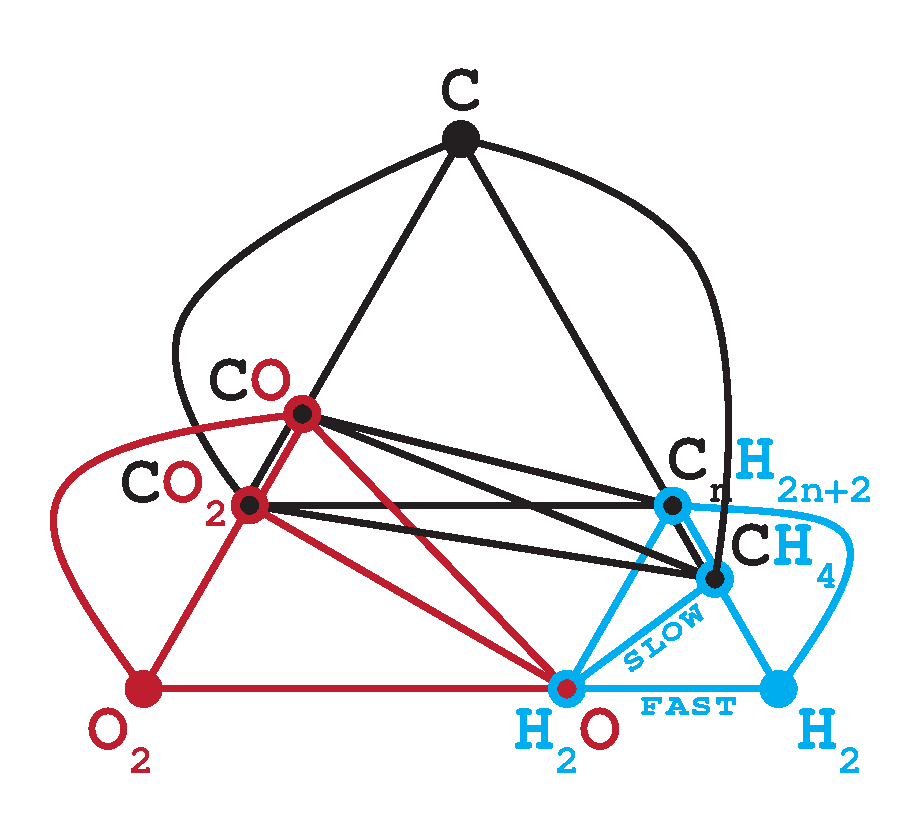
\includegraphics[width=0.4\textwidth]{figures/Fig1.5.pdf}
	\captionsetup{format=myformat}	% hrule beneath caption
	\caption[Pathways for isotopic exchange amongst C--O--H species]{Pathways for isotopic exchange between major species in
		the system C--O--H. The core \& ring of nodes with two colors represent
		the central \& outer atoms, respectively. Each line in this diagram
		represents a geothermometer comprising the isotope ratios of the
		corresponding element in the species at the nodes connected by the line. (Not shown:
		H\textsubscript{3}COOH, H\textsubscript{2}CO, CH\textsubscript{3}OH)}
	\label{fig:1:5}
\end{SCfigure*}